\subsection{Refinement Score Visualization}
\label{app:score_visualization}

Figure~\ref{fig:appendix_refinement_scores} shows the spatial signals used
to construct the sampling policies. PI uses prior information, CPG uses
variation in a coarse prediction, and CA uses a predicted score or a
physical quantity from which the score is computed. For ShapeNet-Car,
the maps show the physical-body prior and the pressure-variation signals
of the Field policies; the full allocation also combines the near-wall
and wake terms specified in Appendix~\ref{app:density_policy_design}.

\begin{figure}[H]
    \centering
    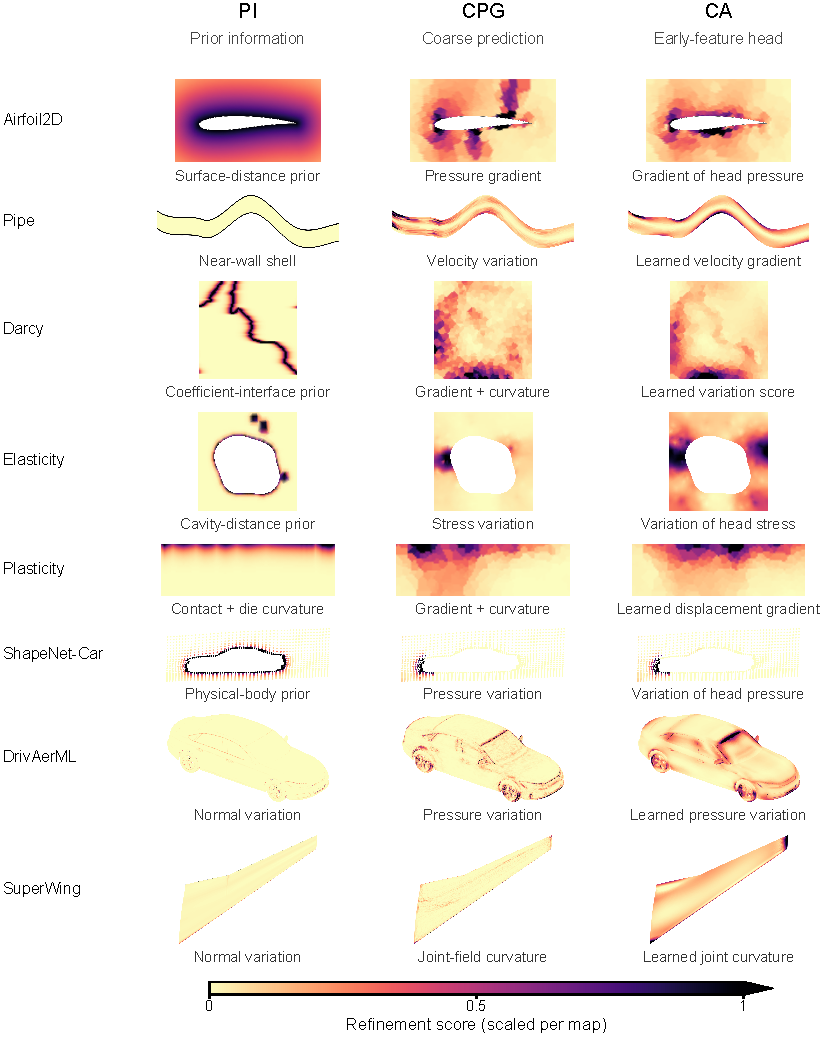
\includegraphics[width=\linewidth,height=.71\textheight,keepaspectratio]{figures/appendix/refinement_score_overview.pdf}
    \caption{\textbf{Refinement scores.} Rows use the eight benchmark cases
    and views of the retained-fraction visualization at a $37.5\%$ budget
    and sampling seed zero. Each map is independently rescaled from its
    minimum to its 99th percentile, with larger values clipped to one.
    Colors progress from pale yellow to dark purple as the score increases.
    Labels identify each signal. Uniform has no refinement score.}
    \label{fig:appendix_refinement_scores}
\end{figure}

\clearpage
\subsubsection{From scores to selected points}
\label{app:score_to_sampling}

Figure~\ref{fig:refinement_score_example} traces one Airfoil case from
the available information through the raw score and sampling weights to
the selected points. Table~\ref{tab:airfoil_score_weights} specifies the
transformations. Here $d_\Gamma$ is the distance to the surface,
$x_{\mathrm{NN}}$ is the nearest coarse point, and $Q_{95}$ is the 95th
percentile over reference points.

\begin{table}[H]
    \centering
    \caption{Raw scores and sampling weights for the Airfoil example.}
    \label{tab:airfoil_score_weights}
    \small
    \renewcommand{\arraystretch}{1.25}
    \begin{tabular}{@{}lcc@{}}
        \toprule
        Policy & Raw score $s(x)$ & Sampling weight $w(x)$ \\
        \midrule
        PI & $\exp(-d_\Gamma(x)/0.3)$ & $1+20s$ \\
        CPG & $\|\nabla_{\mathrm{LSQ},16}\widehat p^{(0)}(x_{\mathrm{NN}})\|_2$
            & $(0.1+s/Q_{95}(s))^2$ \\
        CA & $\|\nabla_{\mathrm{LSQ},16}\widehat p^{\mathrm{head}}(x_{\mathrm{NN}})\|_2$
            & $(0.01+s/Q_{95}(s))^2$ \\
        \bottomrule
    \end{tabular}
\end{table}

Sampling uses the raw scores and weights in
Table~\ref{tab:airfoil_score_weights}. The weights are normalized over
eligible candidates before sampling without replacement. Score colors
use the independent minimum-to-99th-percentile scaling of the overview.

\begin{figure}[H]
    \centering
    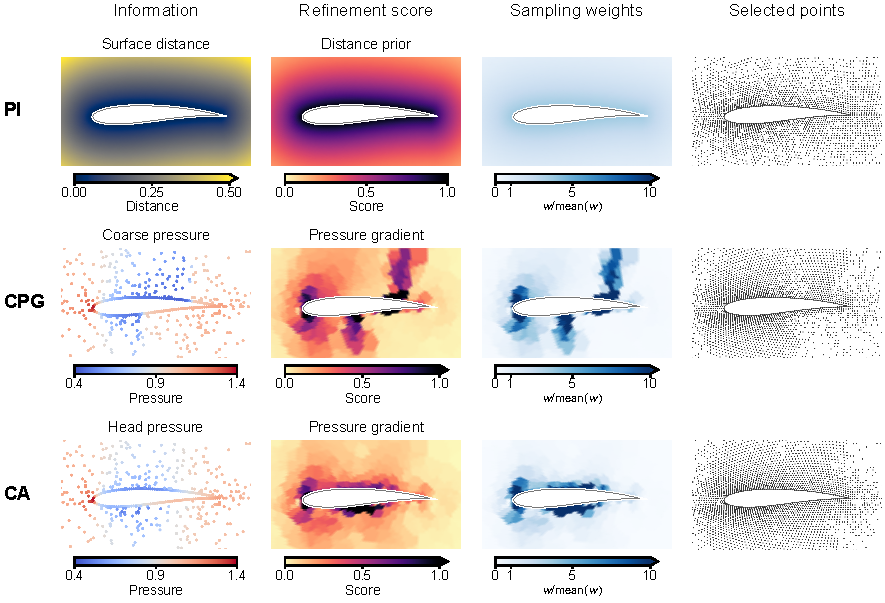
\includegraphics[width=\linewidth]{figures/appendix/refinement_score_example.pdf}
    \caption{\textbf{How scores guide sampling.} Each row shows one policy
    on the same airfoil: input information, refinement score, sampling
    weights, and selected points. Table~\ref{tab:airfoil_score_weights}
    gives the raw-score definitions and sampling transformations.}
    \label{fig:refinement_score_example}
\end{figure}
